%        1         2         3         4         5         6         7         8
\documentclass[letterpaper,10pt,conference]{ieeeconf}

\IEEEoverridecommandlockouts
\overrideIEEEmargins

\usepackage[caption=false,font=footnotesize]{subfig}
\usepackage{graphicx}
\usepackage{booktabs}
\usepackage{array}
\usepackage{algorithm}
\usepackage{algpseudocode}
\usepackage{amsmath}
\usepackage{amssymb}
\usepackage{cite}
\usepackage{xurl}

\makeatletter
\let\NAT@parse\undefined
\makeatother
\usepackage[
    colorlinks=true,
    citecolor=blue,
    linkcolor=blue,
    urlcolor=blue
]{hyperref}

\title{\LARGE \bf
INSERT TITLE HERE
}

\author{INSERT AUTHOR HERE}

\begin{document}

\begin{titlepage}
    \begin{center}
        \vspace*{1cm}
        {\huge INSERT TITLE HERE}
        \vspace{0.5cm}\\
        {\large By}\\
        \vspace{0.5cm}
        \textbf{INSERT AUTHOR HERE}
        \vspace{1.25cm}

        \center{\huge{\textbf{MSc Robotics Final Paper Draft}}}

        \vspace{10mm}
        
\includegraphics[scale=0.6]{logos/bristolcrest_colour.pdf}
        \hspace{5mm}
        
\includegraphics[scale=0.35]{logos/UWE_insignia.png}

        \vspace{10mm}
        {\large School of Engineering Mathematics and Technology\\
        \textsc{University of Bristol}}
        \\
        \&
        \\
        {\large School of Engineering\\
        \textsc{University of the West of England}}\\

        \vspace{0.8cm}
        \begin{minipage}{10cm}
        \center A final paper submitted in accordance with the requirements of the degree of \textsc{Master of Science in Robotics}.
        \end{minipage}\\
        \vspace{0.8cm}
        \today
    \end{center}

    \vspace{0.75cm}
    {\large{Declaration of own work}}

    This draft preserves the frozen research findings and evidence boundary used in the dissertation project. It is a submission draft and should be checked against the required institutional declaration wording before final upload.

    \begin{flushright}
    Name and Date
    \end{flushright}

    \vspace{0.5cm}
    {\large{Ethics statement}}

    \textit{To be confirmed against the dissertation handbook and final submission requirements.}

    \begin{flushright}
    Name and Date
    \end{flushright}

    \vspace{0.35cm}
    {\large{AI disclosure}}

    \textit{AI\_DISCLOSURE\_HUMAN\_REVIEW\_REQUIRED}
\end{titlepage}

\maketitle
\thispagestyle{empty}
\pagestyle{empty}

\begin{abstract}
This paper evaluates whether a structured LLM-assisted decision pipeline can support cooperative control at an unsignalised intersection in SUMO. The controller separates prompt construction, live provider inference, parsing and validation, deterministic fallback, cooperative post-processing, safety verification, and trace logging. The formal evaluation uses a frozen 4-controller, 2-scale, 3-seed design with 24 valid runs, combining the valid 4V \texttt{formal\_v2} evidence and the corrected 8V \texttt{formal\_v4} evidence. Across the retained formal runs, the complete LLM-assisted pipelines achieved lower operational waiting and higher mean speed than the selected rule-based baseline. However, live-provider reliability in the formal experiment was extremely poor, so that traffic advantage cannot be attributed independently to the LLM. A post-hoc 4V seed1 diagnostic with reliable Gemini removed provider failure as a confound and showed no incremental traffic benefit beyond fallback-only: waiting and speed matched the deterministic fallback-only condition, and decision-level agreement was complete. The main contribution is therefore methodological rather than a claim of independent model superiority: a modular, traceable, reproducible framework that exposes pipeline-level behaviour, provider/fallback attribution, and the experimental identifiability limits of LLM-based traffic control.
\end{abstract}

\section{Introduction}
Unsignalised intersection control is a coordination problem: multiple vehicles compete for a shared conflict space, and the controller must balance efficiency, safety, and transparency. SUMO-based microscopic traffic simulation has long supported reproducible evaluation of this setting, while autonomous intersection management has shown that policy design matters as much as motion planning \cite{AlvarezLopez2018,Dresner2008,Safarov2022}. This dissertation asks whether an LLM can be incorporated into such a pipeline in a way that remains reproducible and auditable rather than opaque.

Traditional fixed or rule-based controllers are valuable baselines because they are deterministic, easy to inspect, and easy to reproduce. They are also limited: their behaviour is only as good as the policy rules encoded in advance, and they do not adapt well when the interaction pattern in the conflict space becomes more complex. That limitation makes them a useful benchmark, but also motivates structured decision support when the traffic scene requires context-sensitive reasoning.

The research gap is not simply whether an LLM can emit a structured action. It is whether the performance of the \emph{complete} pipeline can be compared fairly when the system includes parsing, validation, deterministic fallback, cooperative post-processing, and safety verification. Existing LLM-driving work demonstrates the promise of grounded reasoning and modular decision-making \cite{Huang2022,Driess2023,Wen2023,Li2024,Ma2024,Cui2024,Hou2025,Dong2026,Xie2025}, but it does not necessarily separate traffic performance from the independent contribution of successful LLM reasoning.

The contribution of the dissertation is therefore methodological as much as technical: it provides a reproducible SUMO pipeline, a frozen prompt contract, a constrained action interface, and an explicit attribution boundary that allows traffic-level behaviour to be discussed separately from provider reliability and downstream deterministic logic.

The aim of this paper is therefore to evaluate whether a structured LLM-assisted decision pipeline can support cooperative decision-making at an unsignalised intersection while preserving traceability, reproducibility, and deterministic safeguards. Four research questions guide the evaluation:
\begin{itemize}
    \item \textbf{RQ1:} How does the traffic efficiency of the LLM-assisted pipeline compare with the rule-based baseline?
    \item \textbf{RQ2:} Does cooperative post-processing meaningfully change raw LLM behaviour?
    \item \textbf{RQ3:} What effect does deterministic safety verification have on the hybrid pipeline?
    \item \textbf{RQ4:} How does behaviour change from 4 vehicles to 8 vehicles under the tested low-density scenario?
\end{itemize}

The principal contributions are:
\begin{itemize}
    \item a modular LLM-assisted decision architecture for unsignalised intersection control;
    \item traceable provenance that separates raw model output, validation, fallback, post-processing, safety, and final action;
    \item a controlled SUMO evaluation with frozen formal evidence boundaries; and
    \item an attribution analysis that distinguishes pipeline-level behaviour from model-level identifiability.
\end{itemize}

\section{Related Work}
\subsection{Autonomous Intersection and Cooperative Control}
Dresner and Stone \cite{Dresner2008} established the core intersection-management idea that performance depends on the access policy governing a conflict space. Their reservation-based framing is still relevant because it makes the access rule itself part of the research object rather than a hidden implementation detail. Safarov \cite{Safarov2022} extends this logic to unregulated junctions and shows that traffic behaviour depends on the behavioural assumptions encoded in the controller. Taken together, these sources support the view that unsignalised junctions are coordination problems in which policy design, not just motion planning, determines efficiency.

Zhao et al. \cite{Zhao2025} further show that cooperative control at unsignalised intersections can be formulated as an explicit multi-agent coordination problem. That is useful for this dissertation because the controller does not merely choose a single global action; it assigns per-vehicle decisions inside a shared conflict space. The literature therefore motivates a control problem in which the decision rule itself is a first-class object and the interaction among vehicles is part of the evaluation, not a side effect.

The present paper adopts that perspective. Rather than treating the controller as a black box, it makes the decision stages visible so that the effect of each stage can be interpreted separately.

\subsection{LLM Planning and Autonomous Driving}
Huang et al. \cite{Huang2022} show that language models can act as planners, but they also make clear that a plausible plan is not automatically executable. Driess et al. \cite{Driess2023} make the same argument from an embodied multimodal perspective: language reasoning becomes more useful when it is grounded in a structured view of the environment rather than detached text. Wen et al. \cite{Wen2023} reinforce the point through a knowledge-driven autonomous-driving pipeline, which again depends on structured state rather than free-form generation.

Recent autonomous-driving LLM studies \cite{Li2024,Ma2024,Cui2024,Hou2025,Dong2026,Xie2025} strengthen that theme. They suggest that the most defensible use of LLMs is not as unconstrained end-to-end drivers, but as components inside modular pipelines with explicit interfaces, latency constraints, and reliability checks. That is the model adopted in this dissertation: the LLM is a stage in a simulator-facing control architecture, not the sole source of truth.

\subsection{Reliability, Hybrid Control and Research Gap}
The remaining gap is methodological. Existing studies do not always distinguish the behaviour of the full hybrid pipeline from the independent contribution of the model, and reliability-focused work reminds us that plausible output is not the same thing as reliable grounded behaviour \cite{Xie2025}. That distinction matters because provider failure, parser success, fallback handling, and safety logic can dominate the final behaviour.

This is why the dissertation treats the pipeline as an evaluated system rather than treating the model output as the final result. The live provider is only one stage in a larger decision chain. If the live provider is unreliable, then the traffic outcome is the behaviour of a constrained pipeline under provider failure, not a clean measure of model intelligence. That is the methodological problem the dissertation is designed to expose.

This paper therefore evaluates a frozen pipeline and a post-hoc attribution diagnostic separately. The formal experiment answers whether the pipeline performs well; the post-hoc diagnostic asks whether successful live Gemini output adds anything beyond deterministic fallback in the evaluated state.

\section{Methodology}
\subsection{System architecture}
The controller is a staged decision pipeline rather than a single end-to-end model call. SUMO provides the current traffic state and route-conflict context \cite{AlvarezLopez2018}, which are converted into the frozen prompt contract. The live provider returns a candidate action set, which is parsed, validated, and then passed through deterministic fallback, cooperative post-processing, and safety verification before execution. Raw output, validated output, intermediate interventions, and final decisions are all retained in the trace.

\begin{figure*}[t]
\centering
\setlength{\fboxsep}{4pt}
\renewcommand{\arraystretch}{1.15}
\begin{tabular}{c c c c c c c c c}
\fbox{\parbox[c][1.15cm][c]{1.65cm}{\centering \textbf{SUMO state}\\vehicles, routes\\control zone}} &
$\rightarrow$ &
\fbox{\parbox[c][1.15cm][c]{1.70cm}{\centering \textbf{Frozen prompt}\\P1\_BASELINE}} &
$\rightarrow$ &
\fbox{\parbox[c][1.15cm][c]{1.55cm}{\centering \textbf{Live LLM}\\provider call}} &
$\rightarrow$ &
\fbox{\parbox[c][1.15cm][c]{1.70cm}{\centering \textbf{Parser /}\\\textbf{validation}}} &
$\rightarrow$ &
\fbox{\parbox[c][1.15cm][c]{1.80cm}{\centering \textbf{Fallback /}\\\textbf{coop. / safety}}}
\end{tabular}

\vspace{0.5em}

\fbox{\parbox[c][1.0cm][c]{0.26\textwidth}{\centering \textbf{Final action}\\PROCEED / WAIT / FREE}}
\hspace{0.5em}
$\rightarrow$
\hspace{0.5em}
\fbox{\parbox[c][1.0cm][c]{0.46\textwidth}{\centering \textbf{Trace / provenance logging}\\raw, validated, intermediate, and final decisions}}
\caption{Staged LLM-assisted intersection-control pipeline used throughout the dissertation.}
\label{fig:architecture}
\end{figure*}

\begin{table}[t]
\centering
\caption{Controller variants and enabled pipeline stages.}
\label{tab:controllers}
\renewcommand{\arraystretch}{1.08}
\begin{tabular}{p{1.75cm} p{3.5cm}}
\toprule
\textbf{Controller} & \textbf{Enabled stages} \\
\midrule
Rule-Based & Deterministic interface rule only \\
Raw LLM & LLM proposal, parsing, validation, fallback \\
Hybrid & Raw LLM + cooperative post-processing \\
Hybrid + Safety & Hybrid + deterministic safety verification \\
\bottomrule
\end{tabular}
\end{table}

The action space is fixed to \texttt{PROCEED}, \texttt{WAIT}, and \texttt{FREE}. Vehicles outside the control zone are forced to \texttt{FREE}; vehicles inside the conflict zone are evaluated through the canonical prompt and output contract. Importantly, the rule-based baseline is not the same thing as deterministic fallback. The baseline is a standalone controller, whereas fallback is a deterministic policy inside the live LLM pipeline that allows execution to continue when the provider response is unavailable or unusable.

The prompt does not ask the model to invent a new control language. It only asks for one of the three legal actions on the current scene, which keeps the interface compact and makes the downstream parser tractable. That design is deliberate: a smaller action space improves reproducibility, simplifies validation, and makes the comparison against deterministic control easier to interpret.

\subsection{Prompt, parsing and deterministic fallback}
The frozen prompt asks for a structured, per-vehicle decision over the current scene state. The parser and validation layer normalise invalid or missing outputs before execution. This design is intentionally conservative: it protects the simulator from malformed output while preserving a clear record of where a decision came from.

The prompt sees a compact structured representation rather than the raw simulator dump: the relevant vehicle identifiers, route or route-group identity, the vehicle's relation to the control zone, and the local interaction context needed to decide whether it can move. The live provider configuration in the formal experiment was also frozen so that provider reliability could be measured rather than hidden inside changing request behaviour.

The fallback policy has real control semantics. It reasons over route compatibility, conflict structure, and the current movement state to produce a deterministic action when the live model cannot supply a usable one. It is therefore best understood as a second policy, not a mere emergency ``WAIT'' button.

\subsection{Cooperative post-processing and safety verification}
The cooperative stage can promote compatible vehicles when the local scene permits it. The safety verifier checks for conflict violations and can downgrade unsafe actions. These stages are traceable and reproducible, but the formal evidence later shows that they are not strongly exercised in the retained scenarios.

That matters because these stages are not mere logging decorations. They are live parts of the decision pipeline that can change the executed action when the local traffic state makes such a change legal or necessary. In the retained evidence, however, they are best understood as implemented safeguards whose activation is limited by the specific low-density scenarios under test.

\subsection{Reproducibility controls}
The evaluation is frozen by design: prompt contract, model configuration, request configuration, controller semantics, scenario family, vehicle scale, and seeds are fixed before the retained formal comparisons are interpreted. This makes the experiment reproducible and allows the dissertation to distinguish the configured pipeline from the observed results.

Just as importantly, the trace schema retains request identity, provider attempt identity, provider success, parser success, fallback, intermediate decisions, and final decisions. That provenance is what makes the later attribution analysis possible. It answers the question ``what happened inside the pipeline? even when it does not fully answer the harder question ``would the outcome have changed if one stage had been absent?.

\section{Experimental Design}
The formal evaluation uses four controllers, two traffic scales, and three seeds per cell, for a total of 24 valid formal runs. The retained formal evidence combines the valid 4V batch from \texttt{formal\_v2} with the corrected 8V batch from \texttt{formal\_v4}. The nominal 8V \texttt{formal\_v2} traces are excluded because trace validation showed that they loaded the 4-vehicle configuration rather than the intended 8-vehicle scenario.

This is a factorial comparison, not an exploratory sweep. The controller factor addresses RQ1 through RQ3, the scale factor addresses RQ4, and the three seeds provide a descriptive view of variability inside each controller-scale cell. The design therefore supports controlled comparison while still keeping the experiment small enough to remain auditable by hand.

\begin{table}[t]
\centering
\caption{Formal evidence boundary used in the final paper.}
\label{tab:evidence_boundary}
\renewcommand{\arraystretch}{1.08}
\begin{tabular}{p{1.8cm} p{1.6cm} p{1.2cm} p{1.0cm} p{1.35cm} p{1.8cm}}
\toprule
\textbf{Dataset} & \textbf{Controllers} & \textbf{Scale} & \textbf{Seeds} & \textbf{Valid runs} & \textbf{Status} \\
\midrule
formal\_v2 & 4 & 4V+8V planned & 1,2,3 & 12 valid 4V runs & 4V valid, 8V invalid \\
formal\_v4 & 4 & 8V & 1,2,3 & 12 corrected 8V runs & Fully valid 8V evidence \\
Retained evidence & 4 & 4V+8V & 1,2,3 & 24 valid runs & Final dissertation boundary \\
\bottomrule
\end{tabular}
\end{table}

The main traffic metrics are completion rate, operational waiting, mean speed, throughput, and collision count. The pipeline metrics are provider success, parser success, fallback behaviour, latency, post-processing intervention, and safety override. Operational waiting is a proxy defined by stop-like occupancy rather than a classical queueing delay measure, so it should be interpreted consistently but not overclaimed.

Because each controller-scale cell has only three seeds, the results are deliberately descriptive rather than inferential. Mean values and within-cell variation are used to expose the pattern of behaviour, not to claim population-level statistical significance. That is the correct level of interpretation for a frozen dissertation dataset of this size.

\begin{table}[t]
\centering
\caption{Primary research-question to metric mapping.}
\label{tab:rq_metrics}
\renewcommand{\arraystretch}{1.08}
\begin{tabular}{p{0.55cm} p{4.2cm} p{1.7cm}}
\toprule
\textbf{RQ} & \textbf{Primary comparison} & \textbf{Main metric(s)} \\
\midrule
RQ1 & Rule-based vs LLM-assisted pipeline & Waiting, speed \\
RQ2 & Raw LLM vs Hybrid & Waiting, speed, interventions \\
RQ3 & Hybrid vs Hybrid + Safety & Safety overrides, collisions \\
RQ4 & 4V vs 8V robustness & Waiting, speed, fallback \\
\bottomrule
\end{tabular}
\end{table}

The evaluation is descriptive rather than inferential because each controller-scale cell has only three seeds. This is enough for a controlled dissertation comparison, but not enough for strong statistical generalisation.

\section{Results}
Table~\ref{tab:traffic_results} summarises the retained formal traffic evidence. The key pattern is that the complete LLM-assisted pipelines are consistently better than the selected rule-based baseline on the tested traffic metrics, while the LLM-bearing controllers remain similar to one another.

\begin{table*}[t]
\centering
\caption{Formal traffic performance in the retained evidence boundary.}
\label{tab:traffic_results}
\renewcommand{\arraystretch}{1.1}
\begin{tabular}{p{2.75cm} p{0.9cm} p{2.25cm} p{2.05cm} p{1.35cm} p{1.15cm}}
\toprule
\textbf{Controller} & \textbf{Scale} & \textbf{Operational waiting} & \textbf{Mean speed} & \textbf{Completion} & \textbf{Collisions} \\
\midrule
Rule-Based & 4V & 82.0 $\pm$ 0.0 & 2.3098 $\pm$ 0.0000 m/s & 100\% & 0 \\
Rule-Based & 8V & 242.0417 $\pm$ 110.5860 & 1.1895 $\pm$ 0.7540 m/s & 100\% & 0 \\
Raw LLM & 4V & 15.0 $\pm$ 0.0 & 6.8026 $\pm$ 0.0000 m/s & 100\% & 0 \\
Raw LLM & 8V & 15.2917 $\pm$ 2.0450 & 6.5991 $\pm$ 0.2540 m/s & 100\% & 0 \\
Hybrid & 4V & 15.0 $\pm$ 0.0 & 6.8026 $\pm$ 0.0000 m/s & 100\% & 0 \\
Hybrid & 8V & 15.2917 $\pm$ 2.0450 & 6.5991 $\pm$ 0.2540 m/s & 100\% & 0 \\
Hybrid + Safety & 4V & 15.0 $\pm$ 0.0 & 6.8026 $\pm$ 0.0000 m/s & 100\% & 0 \\
Hybrid + Safety & 8V & 15.2917 $\pm$ 2.0450 & 6.5991 $\pm$ 0.2540 m/s & 100\% & 0 \\
\bottomrule
\end{tabular}
\end{table*}

The rule-based baseline degrades sharply from 4V to 8V. The LLM-assisted pipelines remain comparatively stable on the tested scale range. Completion rate saturates at 100\% and collision count remains 0, so the stronger discriminators are operational waiting and mean speed.

\begin{figure*}[t]
\centering
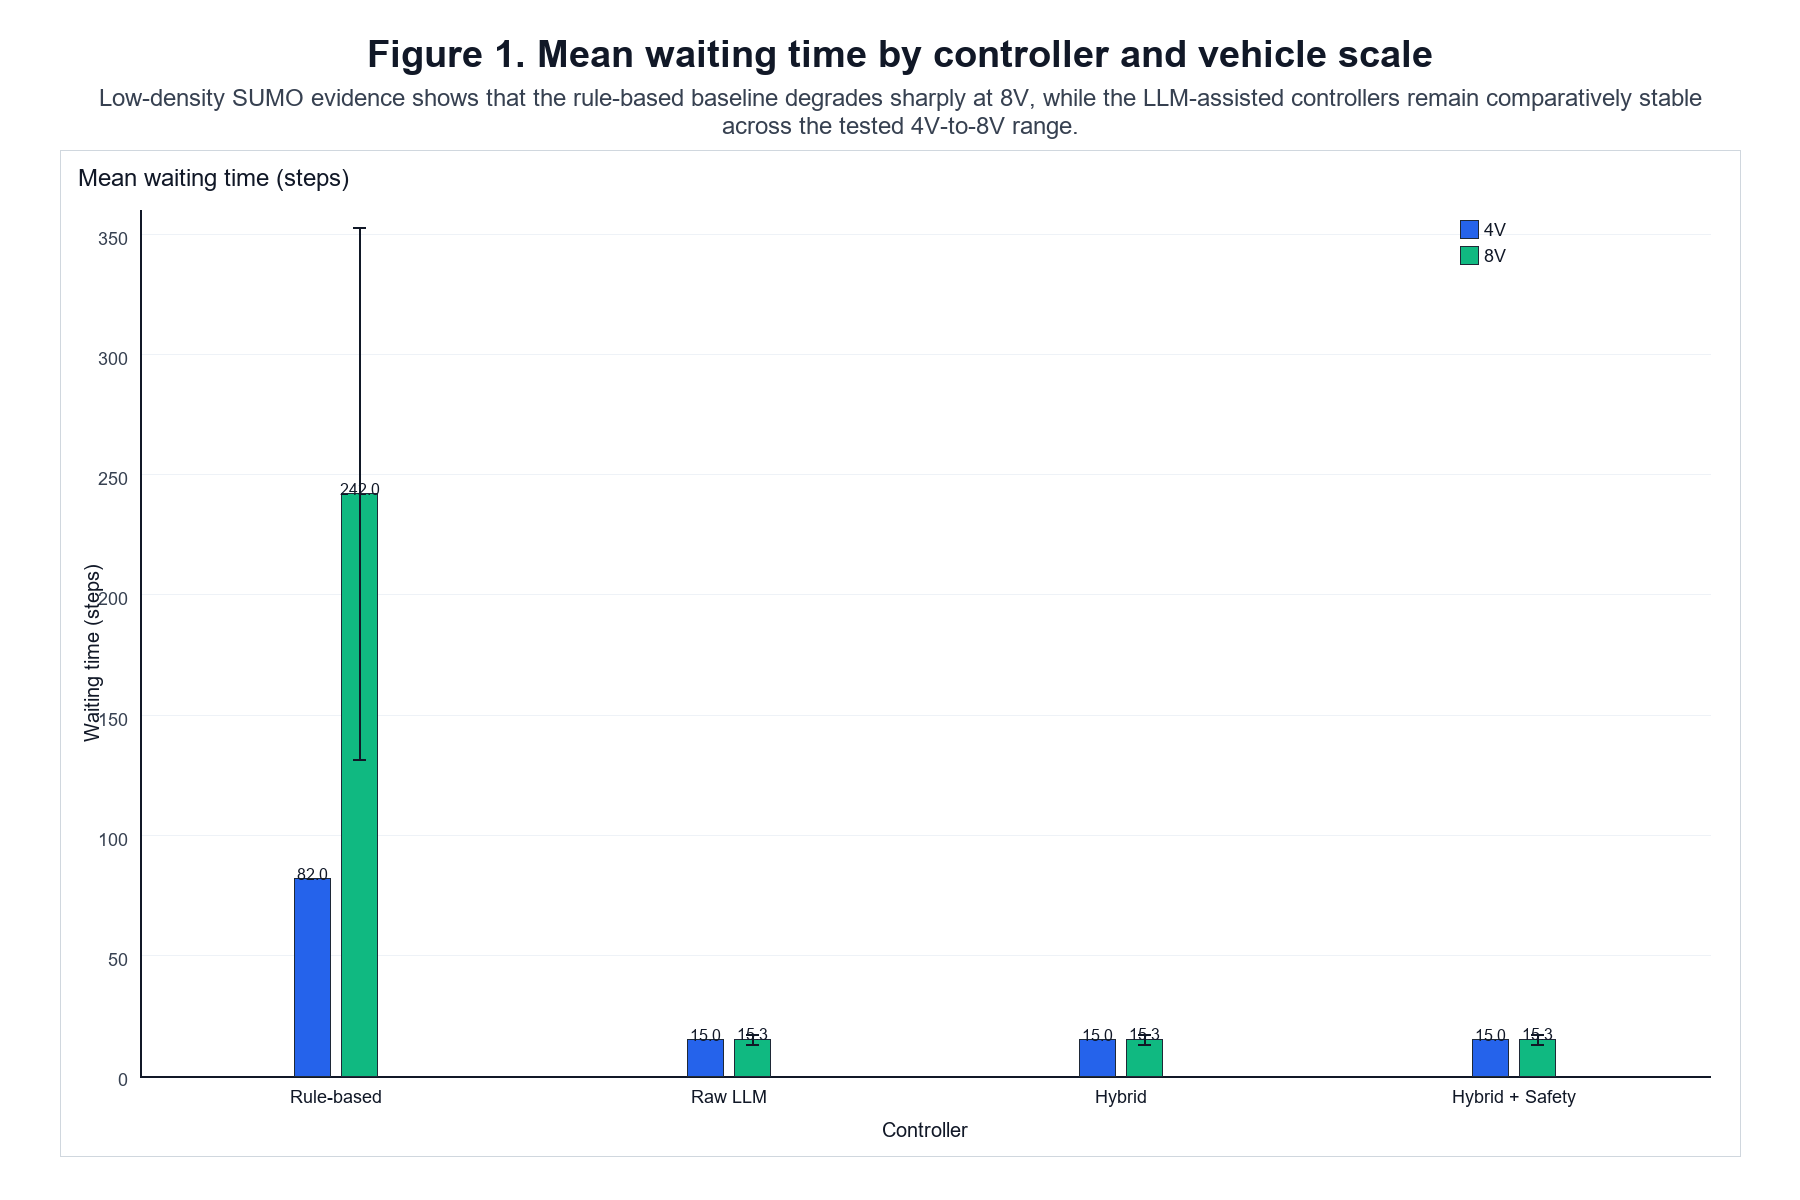
\includegraphics[width=0.48\textwidth]{figures/figure_1_mean_waiting_time.png}
\hfill
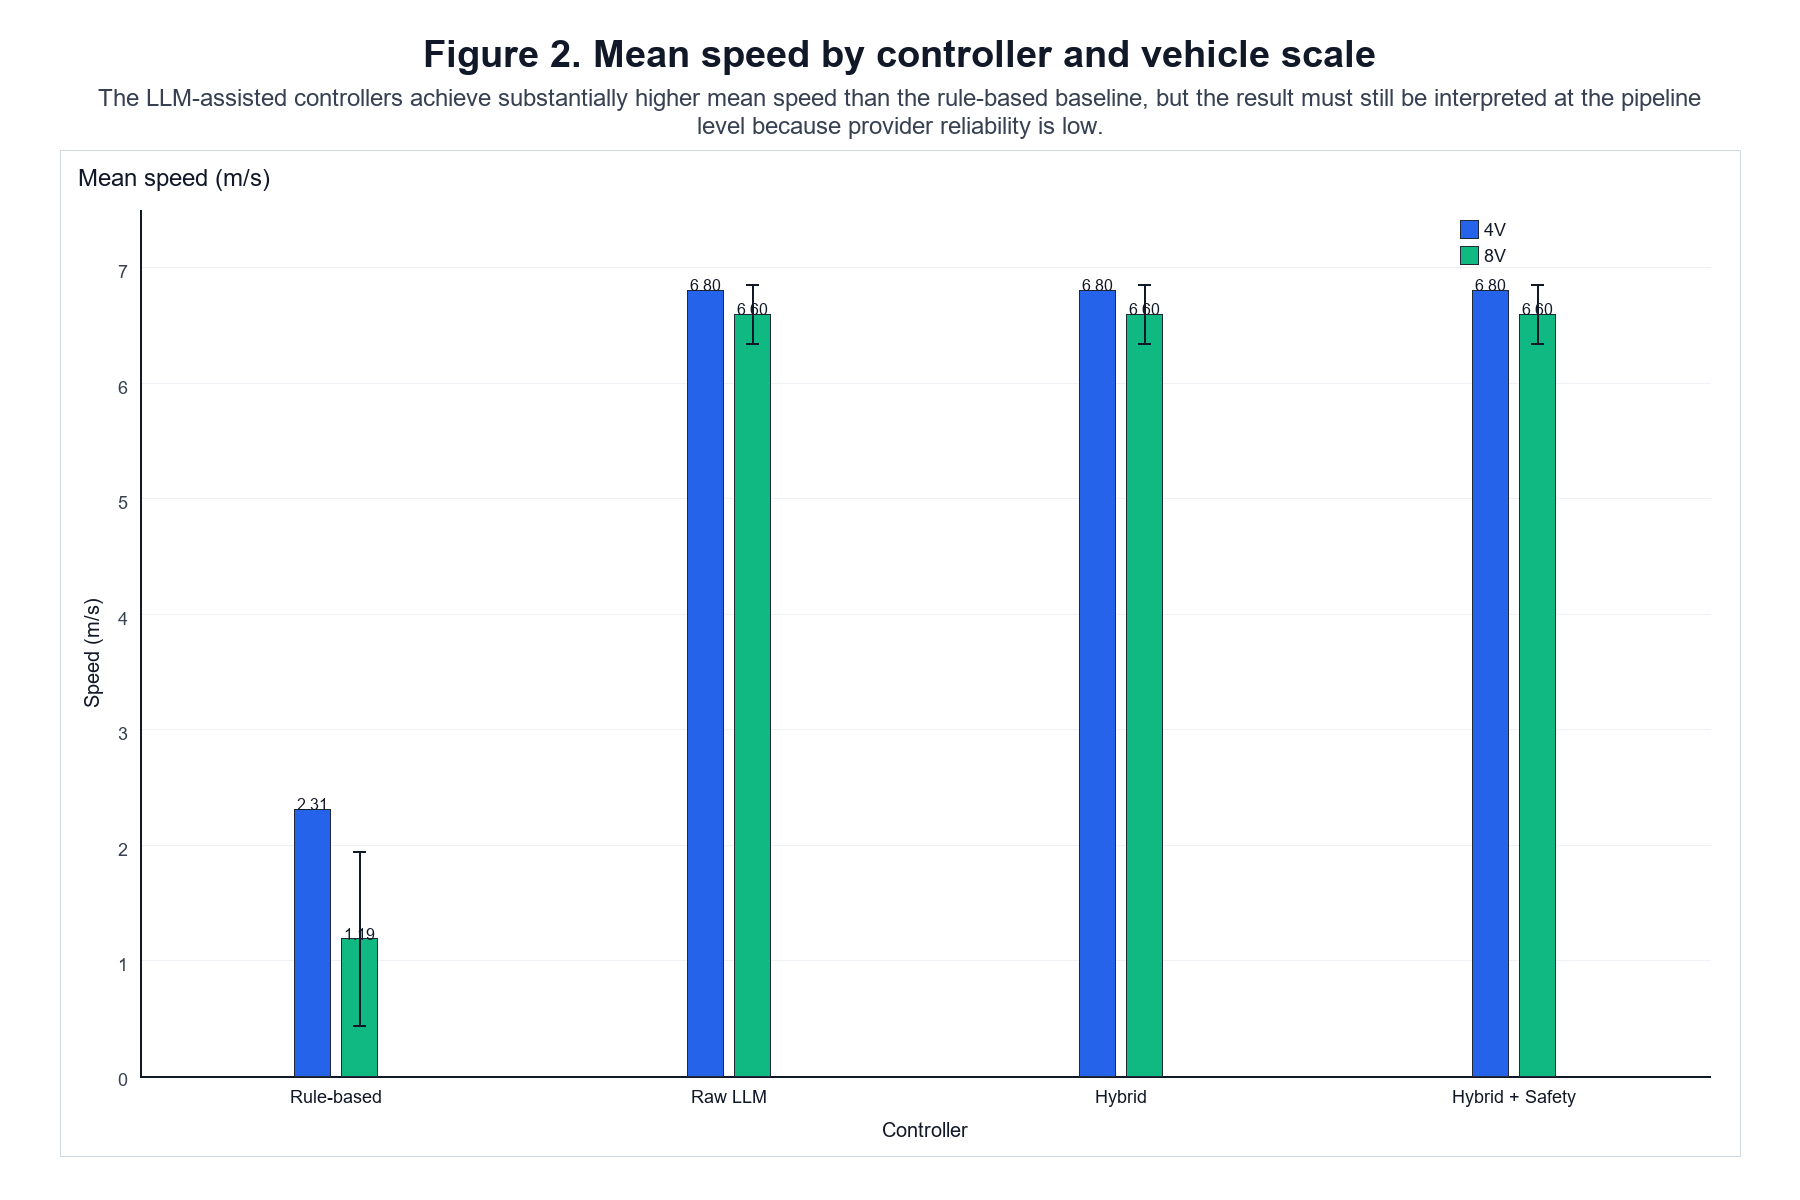
\includegraphics[width=0.48\textwidth]{figures/figure_2_mean_speed.png}
\caption{Descriptive traffic trend plots for operational waiting and mean speed in the retained formal evidence. The plots reproduce the same frozen values reported in Table~\ref{tab:traffic_results} and help visualise the large rule-based to LLM-assisted separation.}
\label{fig:traffic_trends}
\end{figure*}

The plots in Figure~\ref{fig:traffic_trends} are intentionally descriptive rather than inferential. They reinforce the same reading as Table~\ref{tab:traffic_results}: the main separation is between the rule-based baseline and the LLM-assisted pipelines, not among the three LLM-bearing architectures themselves.

\begin{table*}[t]
\centering
\caption{Provider reliability and fallback behaviour in the formal evidence.}
\label{tab:provider_reliability}
\renewcommand{\arraystretch}{1.08}
\footnotesize
\begin{tabular}{p{1.55cm} p{0.82cm} p{1.65cm} p{1.65cm} p{1.65cm} p{1.5cm}}
\toprule
\textbf{Controller} & \textbf{Scale} & \textbf{Attempts} & \textbf{Successes} & \textbf{Success rate} & \textbf{Mean latency} \\
\midrule
Raw LLM & 4V & 53.000 $\pm$ 0.000 & 3.333 $\pm$ 4.714 & 6.29\% $\pm$ 8.89\% & 101.412 $\pm$ 29.695 ms \\
Raw LLM & 8V & 106.333 $\pm$ 0.471 & 0.667 $\pm$ 0.471 & 0.63\% $\pm$ 0.44\% & 76.846 $\pm$ 1.552 ms \\
Hybrid & 4V & 53.000 $\pm$ 0.000 & 3.000 $\pm$ 4.243 & 5.66\% $\pm$ 8.00\% & 111.021 $\pm$ 23.614 ms \\
Hybrid & 8V & 106.333 $\pm$ 0.471 & 0.333 $\pm$ 0.471 & 0.31\% $\pm$ 0.44\% & 79.035 $\pm$ 4.074 ms \\
Hybrid + Safety & 4V & 53.000 $\pm$ 0.000 & 3.000 $\pm$ 4.243 & 5.66\% $\pm$ 8.00\% & 96.152 $\pm$ 22.919 ms \\
Hybrid + Safety & 8V & 106.333 $\pm$ 0.471 & 0.333 $\pm$ 0.471 & 0.31\% $\pm$ 0.44\% & 76.398 $\pm$ 1.312 ms \\
\bottomrule
\end{tabular}
\end{table*}

Provider reliability is therefore a first-order validity threat. The traffic outcomes should be interpreted as the behaviour of the full pipeline under constrained provider availability rather than as isolated model performance.

\begin{figure*}[t]
\centering
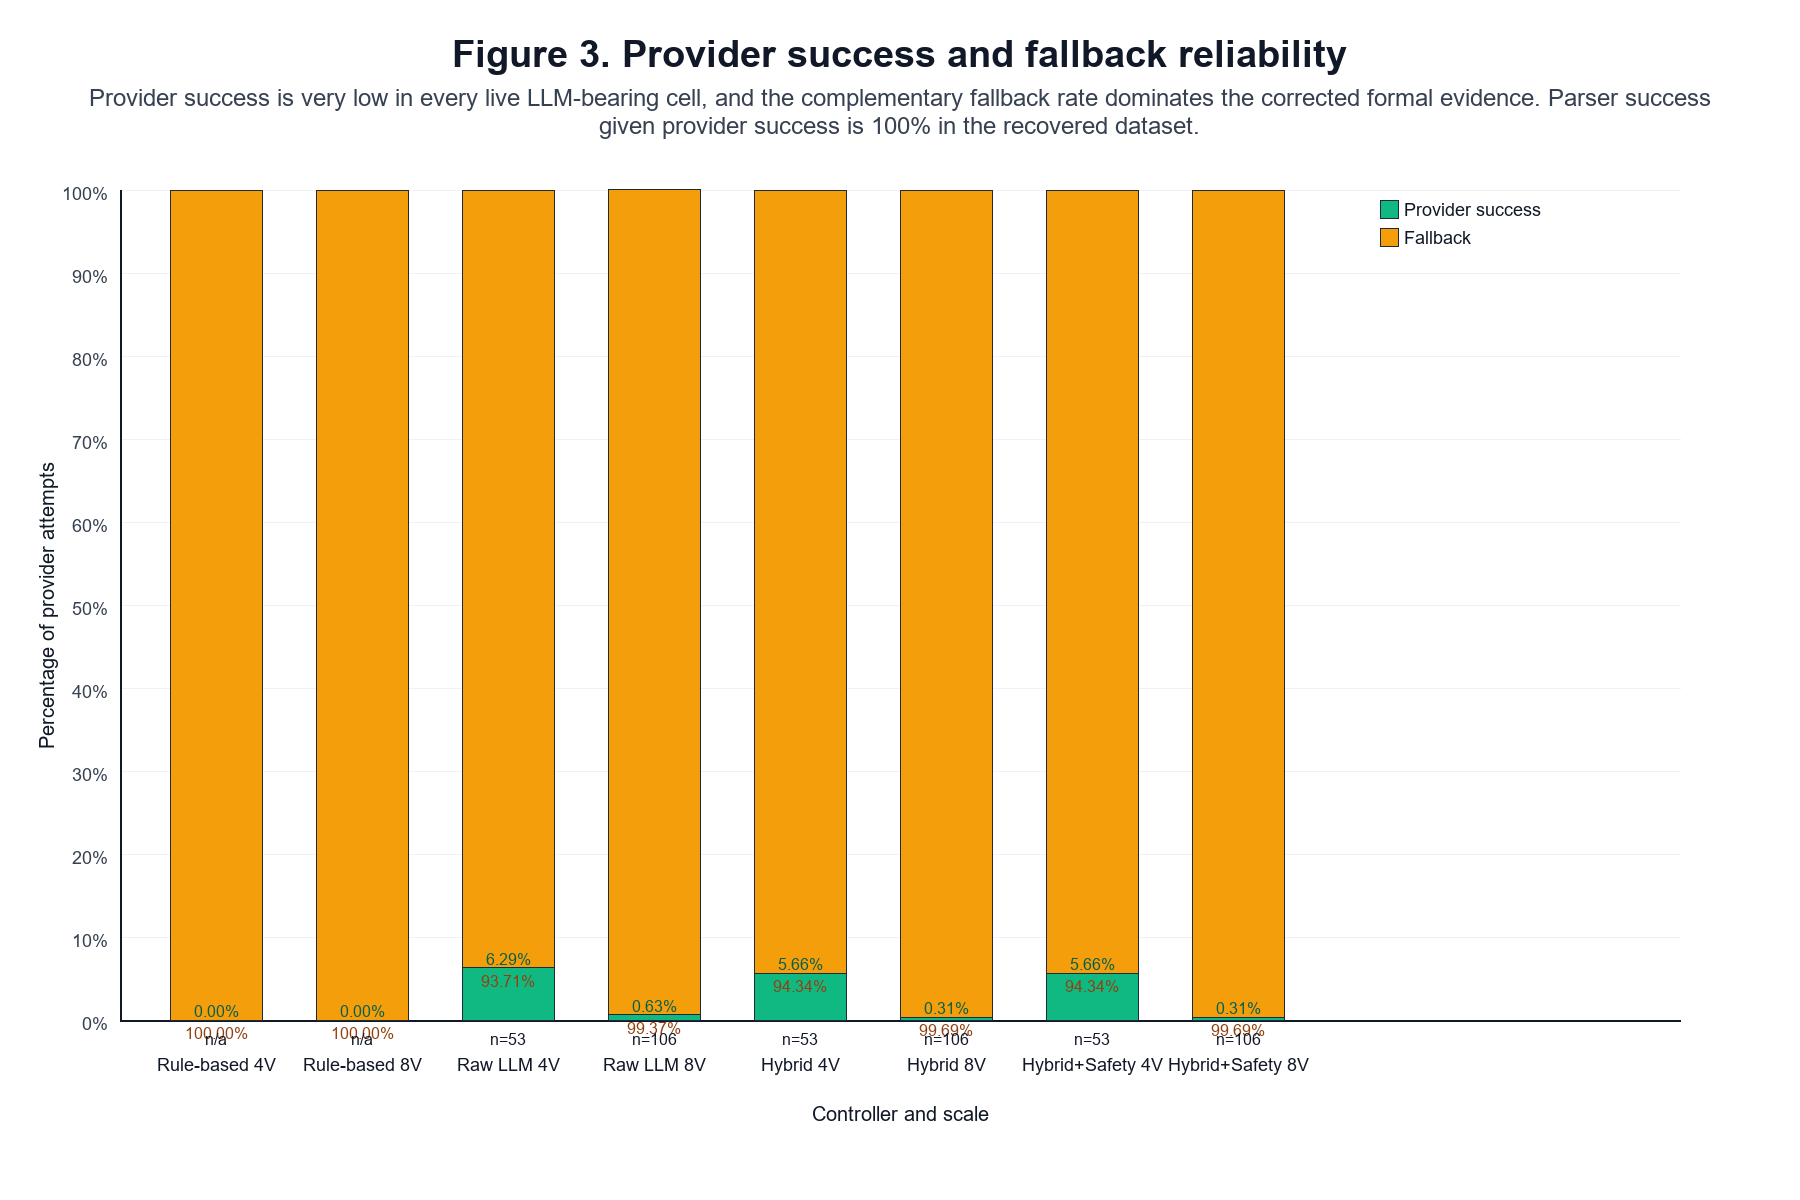
\includegraphics[width=0.48\textwidth]{figures/figure_3_provider_success_fallback.png}
\hfill
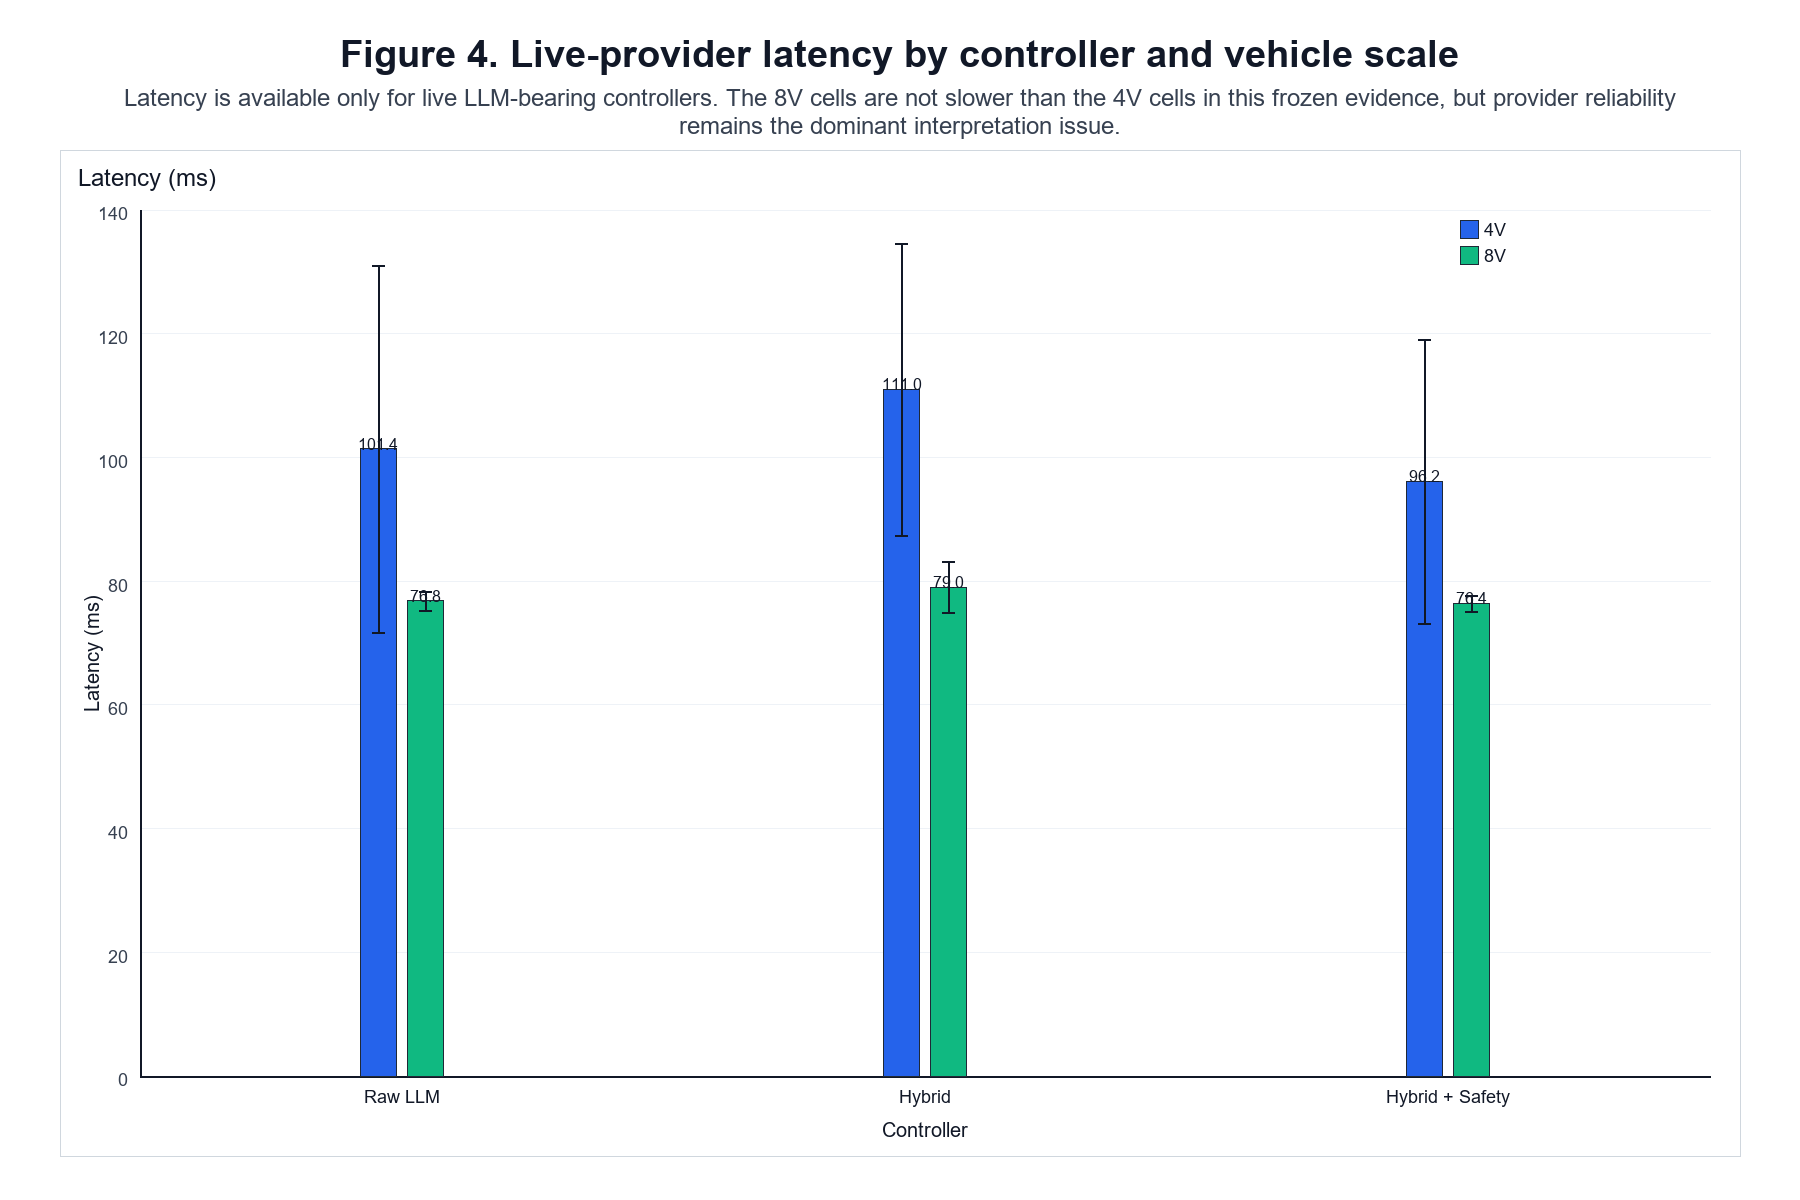
\includegraphics[width=0.48\textwidth]{figures/figure_4_latency.png}
\caption{Provider reliability and latency summaries for the formal live-provider runs. The left plot shows the strong fallback dominance, while the right plot shows the long-tail latency variation that accompanies the unreliable live-provider path.}
\label{fig:provider_path}
\end{figure*}

The reliability plots in Figure~\ref{fig:provider_path} make the same point visually: the live provider path is both sparse and variable, so the formal traffic result cannot be read as if the LLM were directly controlling every decision.

\begin{table}[t]
\centering
\caption{Post-hoc attribution evidence for the reliable Gemini 4V seed1 diagnostic.}
\label{tab:attribution}
\renewcommand{\arraystretch}{1.08}
\footnotesize
\begin{tabular}{p{1.9cm} p{1.55cm} p{1.1cm} p{1.2cm} p{1.9cm}}
\toprule
\textbf{Condition} & \textbf{Provider path} & \textbf{Waiting} & \textbf{Mean speed} & \textbf{Decision agreement} \\
\midrule
Reliable Gemini 4V seed1 & 53/53 success, 0 fallback & 11.0 & 7.58 m/s & 132/132 raw and final \\
Fallback-only 4V seed1 & deterministic fallback only & 11.0 & 7.58 m/s & matched action stream \\
High-discrimination subset & same diagnostic slice & -- & -- & 39/39 raw and final \\
\bottomrule
\end{tabular}
\end{table}

This post-hoc diagnostic is supplementary evidence. It removes provider failure as a confound, but it does not add incremental traffic benefit beyond fallback-only in the evaluated 4V seed1 state.

The important point is that the post-hoc condition strengthens the attribution argument rather than the traffic argument. It shows that once provider reliability is no longer the bottleneck, the reliable Gemini path still collapses back to the same executed actions and the same traffic outcome as fallback-only. That is exactly why the paper separates formal evidence from post-hoc attribution evidence.

\section{Discussion and Limitations}
\subsection{RQ1: pipeline-level advantage, not independent LLM superiority}
The formal evidence supports a pipeline-level traffic advantage: the complete LLM-assisted pipelines show lower waiting and higher speed than the selected rule-based baseline in the tested scenarios. However, because formal provider reliability is extremely poor, the observed result cannot be attributed independently to the LLM. The right claim is about the pipeline, not about model superiority.

That distinction is consistent with the literature on autonomous intersection management and modular LLM-based systems: the system can be better than a rule-based benchmark while still failing to establish that the live model alone caused the gain. In other words, the dissertation supports a pipeline-level improvement claim, but not a clean model-level superiority claim.

\subsection{RQ2 and RQ3: no measurable independent benefit from hybrid or safety layers}
The corrected evidence does not show a measurable traffic advantage for the Hybrid controller over Raw LLM, and it does not show an independent safety-verifier effect. Both stages are present, traceable, and reproducible, but they are not sufficiently exercised in the retained formal scenarios to support a stronger causal claim.

That should not be read as a negative result about the implementation itself. It is a result about the evidence boundary: the architecture contains the additional stages, but the retained scenarios do not create enough disagreement for those stages to reveal a distinct traffic effect. The safest conclusion is therefore one of non-discrimination, not one of architectural failure.

\subsection{RQ4 and the 4V-to-8V interpretation}
The system remains comparatively stable from 4V to 8V in the evaluated low-density setting, but this is not a general scalability result. It is only evidence that the tested pipeline remained operational within the frozen 4V and 8V boundary. The dissertation therefore supports robustness within the tested range, not a universal scalability claim.

This aligns with the broader literature in a careful way. Prior work motivates modular, grounded, reliability-aware pipeline design, but the present study adds the narrower point that stability inside a small low-density range is not the same thing as scalability in the general autonomous-driving sense. The claim must therefore stay local to the tested intersection and vehicle counts.

\subsection{Two separate attribution limitations}
The main methodological contribution of the paper is the distinction between two different limitations:
\begin{itemize}
    \item \textbf{Provider reliability:} the live provider failed often enough that fallback dominated the formal experiment.
    \item \textbf{Behavioural identifiability:} even when Gemini was reliable, the diagnostic condition reproduced the fallback-only traffic outcome and decision stream.
\end{itemize}

Together these mean that traceability is not the same as causal identifiability. The dissertation can say what the pipeline did, but the formal evidence alone cannot isolate the independent contribution of live LLM reasoning.

The post-hoc Gemini diagnostic makes that distinction concrete: even when the provider is reliable and the provenance is complete, the executed action stream still matches fallback-only. That is a stronger result than a logging exercise because it shows that adding more reliable model calls is not sufficient, by itself, to create a different behavioural outcome.

\subsection{Limitations}
The study is limited to 4V and 8V, three seeds per cell, a single low-density SUMO intersection, and an operational waiting proxy rather than a full queueing measure. Prompt/fallback semantic overlap also makes it difficult to separate LLM-specific effect from deterministic policy effect. The cooperative and safety mechanisms are present, but the corrected evidence shows that they are insufficiently activated to support strong positive claims.

\section{Conclusion}
The paper presents a modular, traceable LLM-assisted control pipeline for unsignalised intersection management in SUMO. The formal 24-run evidence shows a pipeline-level traffic advantage over the selected rule-based baseline, while the post-hoc Gemini diagnostic shows no incremental benefit beyond fallback-only in the evaluated 4V condition.

What can be claimed is therefore bounded but meaningful: the architecture is reproducible, the pipeline-level comparison is valid, and the attribution boundary is explicit. What cannot be claimed is independent LLM superiority, general scalability, safety superiority, or a standalone cooperative benefit.

Future work should prioritise causal identification, discriminative scenarios, stronger component ablation, larger and more complex traffic settings, reliable provider or local-model comparison, and real-world or hardware-in-the-loop validation.

\bibliographystyle{IEEEtran}
\bibliography{References}

\end{document}
